\documentclass{standalone}
\usepackage{tikz}
\begin{document}
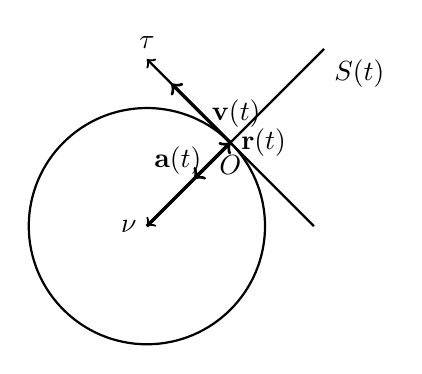
\begin{tikzpicture}[scale=1.5]
    \coordinate (O) at(0,0);
    \node[below] at(0.707, 0.68) {$O$};
    \draw[->, thick] (1.414,0)--(0,1.414)node[above]{$\tau$};
    \draw[->, thick] (1.5, 1.5)node[below right]{$S(t)$}--(O)node[left]{$\nu$};

    \draw[thick](0,0)circle(1);
    

    \coordinate (r) at (0.707, 0.707);
    \coordinate (tau) at (0.4, 0.4);
    \coordinate (nu) at (0.4, 0.4);


    \draw[->,very thick] (O)--(r) node[right]{$\mathbf{r}(t)$};
    \draw[->,very thick] (r)--(0.207,1.207)node[midway, right]{$\mathbf{v}(t)$};
    \draw[->,very thick] (r)--(nu) node[midway, left]{$\mathbf{a}(t)$};
\end{tikzpicture}
\end{document}